\section{氢气的性质和用途}\label{sec:2-3}

\subsection{氢气的性质}

1. 氢气的物理性质

在通常状况下,氢气是一种没有颜色、没有气味的气体。
在 $1$ 标准大气压下,氢气在 $-252.4$ ℃ 时,能变成无色的液体,
在 $-259.1$ ℃ 时,能变为雪状的固体。它难溶于水。

我们已经知道,氢气是最轻的气体。除了已知可用向下排空气法收集氢气外,
还可以用什么方法证明氢气比同体积的空气轻呢?

\begin{shiyan}
    装置如图 \ref{fig:2-7} 所示。球形干燥管里装有碱石灰干燥剂。
    导管口蘸些肥皂水\footnote{肥皂水可用肥皂或洗衣粉配制,可加少量甘油。}。
    调节启普发生器的导气管,控制氢气流速,吹出肥皂泡。
    当肥皂泡吹到足够大时,轻轻摆动导管,让肥皂泡脱管口,
    这时可以观察到什么现象?
\end{shiyan}

从上面的实验可以看到,肥皂泡迅速上升。这说明氢气比空气轻。
据测定,在标准状况下,$1$ 升氢气的质量是 $0.0899$ 克。
氢气跟同体积的空气相比,质量约是空气的 $1/14$。
这就是可以用向下排空气法收集氢气的原因。

\begin{figure}[htbp]
    \centering
    \begin{minipage}[b]{7cm}
        \centering
        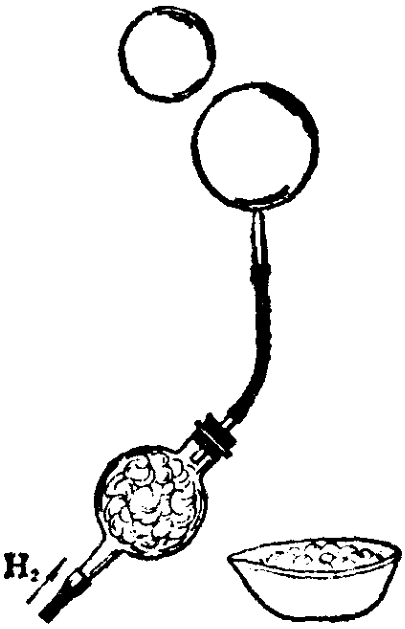
\includegraphics[width=4cm]{../pic/czhx1-ch2-7}
        \caption{氢气流吹肥皂泡}\label{fig:2-7}
    \end{minipage}
    \qquad
    \begin{minipage}[b]{7cm}
        \centering
        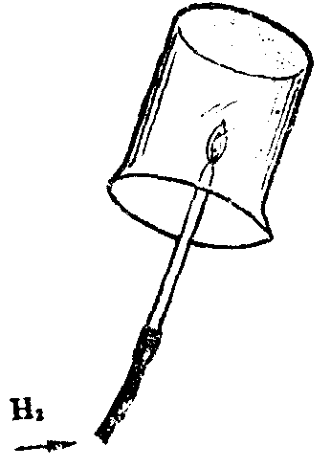
\includegraphics[width=4cm]{../pic/czhx1-ch2-8}
        \caption{氢气在空气里燃烧}\label{fig:2-8}
    \end{minipage}
\end{figure}

2. 氢气的化学性质

氢气在常温下性质隐定,但在点燃或加热等条件下,能够跟许多物质发生化学反应。

(1) 氢气的可燃性

\begin{shiyan}
    在带尖嘴的导管口点燃纯净的氢气,观察火焰的颜色。
    然后在上方罩一个冷而干燥的烧杯(图 \ref{fig:2-8} ),过一会儿,观察烧杯壁上有什么现象发生。
\end{shiyan}

纯净的氢气在空气里安静地燃烧,产生淡蓝色火焰\footnote{氢气在玻璃导管口燃烧,火焰稍带黄色。},
烧杯壁上有水珠生成,接触烧杯的手能感到发烫。
这是由于氢气跟空气里的氧气发生反应,生成了水并放出大量的的热。
\begin{fangchengshi}
    \ce{ 2 H2 + O2 \xlongequal{\text{点燃}} 2 H2O }
\end{fangchengshi}

如果氢气不纯,混有空气(或氧气),点燃时会怎样呢?


\begin{figure}[htbp]
    \centering
    \begin{minipage}[b]{7cm}
        \centering
        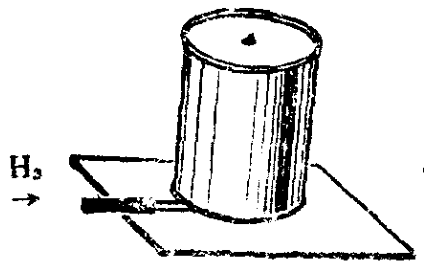
\includegraphics[width=6cm]{../pic/czhx1-ch2-9-1}
        \caption*{I}
    \end{minipage}
    \qquad
    \begin{minipage}[b]{7cm}
        \centering
        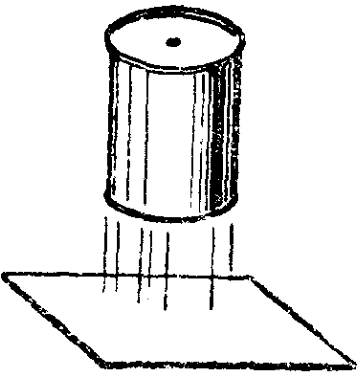
\includegraphics[width=5cm]{../pic/czhx1-ch2-9-2}
        \caption*{II}
    \end{minipage}
    \caption{氢气与空气混和点燃发生爆炸}\label{fig:2-9}
\end{figure}


\begin{shiyan}
    取一个一端开口、另一端钻有小眼的纸筒(或铁罐头筒),用纸团(或手指)堵住小眼,
    通入氢气一会儿(图 \ref{fig:2-9}, I),以使纸筒内充满氢气与空气的混和气体。
    关闭启普发生器的导气管活塞,并将启普发生器移开,拿掉堵眼的纸团(或移开手指),
    用燃着的木条在小眼处点火、注意有什么现象发生。
    (做这个实验时要离人远点,注意安全。)
\end{shiyan}

在这个实验里点火后将听到砰然巨响,爆炸的气浪把纸筒(或铁罐头筒)高高掀起(图 \ref{fig:2-9},II)。

为什么同样是氢气跟空气里的氧气起反应,纯净的氢气能安静地燃烧,而混和气体却发生爆炸?
这是因为当纯净的氢气燃烧时,它的分子只在导管口跟氧气分子接触并发生反应,那里氢气分子少,
跟氧气分子接触也少,产生的热量也小,而且热量很快就散失在空气中;
但在混和气体里却是大量的氢气分子跟氧气分子充分接触,点燃后二者迅速发生反应,
在极短的时间内放出大量的热,气体体积在一个受限制的空间内急剧膨胀,就发生爆炸。
这个反应在上述大口的容器内进行,气体冲出容器,激动空气,只发生爆鸣,并没有什么危险。
如果反应在密闭的或容积大而口小的容器内进行,气体不能排出或来不及排出,就会炸破容器,发生危险。

实验测定,空气里如果混入氢气的体积达到总体积的 4—74.2\% 这个范围,点燃时就会爆炸。
这个范围叫做爆炸极限。因此,我们在\zhongdian{使用氢气时,要特别注意安全。
点燃氢气前,一定先要检验氢气的纯度。}

\begin{shiyan}
    用排水法收集一试管氢气,用拇指堵住,移近火焰,移开拇指点火,如果听到尖锐的爆鸣声,
    就表明氢气不纯,需要再收集,再检验,直到响声很小,才表明氢气已纯净。
    如果用向下排空气法收集氢气,经检验不纯而需要再检验时,应该用拇指堵住试管口一会儿,
    然后再收集氢气检验纯度,否则会发生危险,为什么\footnotemark ?
\end{shiyan}
\footnotetext{
    因为刚检验过纯度的试管内,氢气火焰可能还没有熄灭,如果立刻就用这个试管去收集氢气,
    氢气火焰可能会点燃氢气发生器里尚混有空气的氢气,使氢气发生器发生爆炸。
    用拇指堵住试管口一会儿,能使试管内未熄灭的氢气火焰因缺氧气而熄灭。
}

氢气不仅能在氧气里燃烧,而且还能在一种叫做氯气(\ce{Cl2})的气体里燃烧。

\begin{shiyan}
    如图 \ref{fig:2-10} 所示,先在空气里点燃氢气,然后把导管伸进有黄绿色氯气的瓶里,
    观察氢气在氯气里燃烧时火焰的颜色。
\end{shiyan}

氢气在氯气里继续燃烧,并发出苍白色的火焰,同时产生大量的热。
燃烧后生成的气体是氯化氢(\ce{HCl})。它在空气里易跟水蒸气结合,呈现雾状。
这个反应可以用化学方程式表示如下:
\begin{fangchengshi}
    \ce{ H2 + Cl2 \xlongequal{\text{点燃}} 2 HCl }
\end{fangchengshi}
氯化氢溶解于水即得盐酸。

从上面氢气在氯气中燃烧的反应可以看出,燃烧不一定要有氧气参加。
因此,任何发热发光的剧烈的化学反应,都可以叫做燃烧。

\begin{figure}[htbp]
    \centering
    \begin{minipage}[b]{7cm}
        \centering
        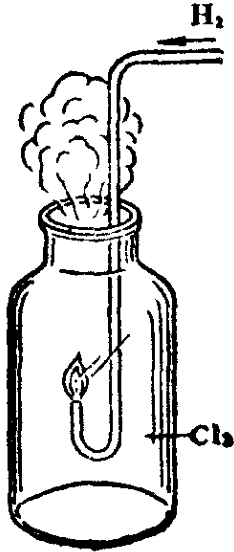
\includegraphics[width=2cm]{../pic/czhx1-ch2-10}
        \caption{氢气在氯气里燃烧}\label{fig:2-10}
    \end{minipage}
    \qquad
    \begin{minipage}[b]{7cm}
        \centering
        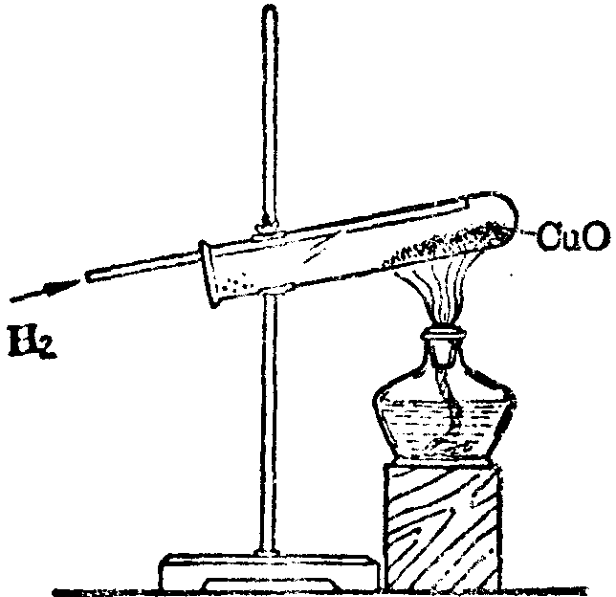
\includegraphics[width=5cm]{../pic/czhx1-ch2-11}
        \caption{氢气还原氧化铜}\label{fig:2-11}
    \end{minipage}
\end{figure}

(2) 氢气的还原性

氢气不但能跟游离态的氧起反应,而且能跟某些氧化物里的氧起反应。
这是氢气的另一个重要化学性质。现在用氢气跟氧化铜(\ce{CuO})的反应为例来说明。

\begin{shiyan}
    在干燥的硬直试管底部铺一层黑色的氧化铜,管口微向下倾斜(图 \ref{fig:2-11})。
    通入氢气,过一会儿再给氧化铜加热。注意观察黑色氧化铜有什么变化,
    管口有什么生成。反应完后停止加热,还要继续通入氢气,直到试管冷却。为什么?
\end{shiyan}

氧化铜由黑色逐渐变为光亮的红色,同时管口有水滴生成。
这就是说,氢气夺取了氧化铜里的氧,跟它化合成水,氧化铜失去了氧,变成红色的金属铜。
这个反应可用化学方程式表示如下:
\begin{fangchengshi}
    \ce{ H2 + CuO \xlongequal{\Delta} Cu + H2O }
\end{fangchengshi}

在这个反应里,氧化铜失去了氧而变成游离态的铜,我们说氧化铜被还原。
这种含氧化合物里的氧被夺去的反应,叫做\zhongdian{还原反应}。
氢气是使氧化铜还原为铜的物质,象这种使含氧化合物发生还原反应的物质就叫做\zhongdian{还原剂}。
因此,氢气具有还原性。


\subsection{氧化-还原反应}

在上面的反应里,从氧化铜来说,它发生了还原反应。
但是从氢气来说,它跟氧化铜中的氧起反应生成了水,发生了氧化反应。
这两个截然相反的过程是在一个反应里同时发生的。
因为在这一类反应里,有一种物质跟氧化合,必然同时有另一种物质里的氧被夺取。
也就是说,有一种物质被氧化,必然有另一种物质被还原。象这样%
\zhongdian{一种物质被氧化,同时另一种物质被还原的反应,叫做氧化-还原反应。}
氢气使氧化铜还原的反应就是氧化-还原反应。
\begin{fangchengshi}
    \phantom{a} \\[1em]
    \ce{ CuO + H2 \xlongequal{\Delta} Cu + H2O }
    \tikz [overlay, >=Stealth] {
        \draw [->] (-3.8,  0.4) -- (-3.8,  0.7) -- (-1.5,  0.7) node [midway, above] {\small 被还原} -- (-1.5,  0.4);
        \draw [->] (-2.7, -0.1) -- (-2.7, -0.5) -- (-0.4, -0.5) node [midway, below] {\small 被氧化} -- (-0.4, -0.1);
    }
    \\[1em]
\end{fangchengshi}

我们已经知道,能夺取含氧化合物里的氧,使含氧化合物发生还原反应的物质叫做还原剂。
由此可以推断,能供给氧,使别种物质发生氧化反应的物质叫做\zhongdian{氧化剂}。
在上述反应里,氧化铜是氧化剂,它具有氧化性。



\subsection{自然界里的氢和氢气的用途}

在自然界里,游离态的氢很少,化合态的氢却很多。氢在水的成分里,按质量计算,约占 $11\%$。
一切生物的细胞组织成分里都含有氢。石油、天然气和煤里也含有氢。

氢气有许多有用的性质,所以有广泛的用途。
氢气密度小,可以用来充灌研究高空气象的探空气球。

由于氢气跟氧气反应放出大量的热,氢气在氧气中燃烧的火焰——氢氧焰可达 $3000$ ℃ 的高温。
生产上用氢氧焰焊接或割断金属,熔化熔点很高的石英,制成各种石英制品。
液态氢还可以做火箭或导弹的高能燃料。氢气用来作一般的燃料,也有十分突出的优点:
资源十分丰富,燃烧时发热量高(每公斤氢气燃烧放热 $34000$ 千卡,热量是汽油的 $3$ 倍),
生成的产物是水,污染少。所以近年来对氢气作为新型燃料的研究很重视。
今后如能在利用太阳能和水制取氢气的技术上有所突破,得到便宜而丰富的氢气,
那么,氢气将成为一种重要的新型燃料。

利用氢气的还原性,冶金工业可冶炼钨、钼等重要金属,电子工业可制取半导体材料高纯硅,
焊接工艺为防止金属在高温下发生氧化,可用氢气作为还原性保护气。

大量的氢气还用在化学工业方面。例如,制造氨(\ce{NH3})和盐酸等重要化工产品都需要氢气做原料。



\begin{xiti}

\xiaoti{列表比较氢气和氧气的物理性质和化学性质。}

\xiaoti{填空:用排空气法收集比空气重的气体,集气瓶的口应向 \xhx,这叫做向 \xhx 排空气法;
    收集比空气轻的气体,集气的口应向 \xhx, 这叫做向 \xhx 排空气法。
}

\xiaoti{一个学生在检验氢气纯度的时候,把收集了氢气的试管管口向上(没堵口)移近火焰,
    结果没有爆鸣声,他判断氢气已经纯净了。另一个学生进行检验时听到了尖锐的爆鸣声,
    他未采取任何措施,打算马上就用这支试管去收集氢气,进行第二次检验。
    他们的操作方法有没有不正确的地方?第一个学生的判断有没有错误?
    第二个学生的操作可能会造成什么后果?
}


\xiaoti{用氢气还原氧化铜的实验,为什么要通一会儿氢气再加热?
    反应完毕撤火后,为什么还要继续通氢气至试管冷却?
}


\xiaoti{用化学方程式表示下列两个在高温下进行的反应,并指出什么物质是氧化剂,什么物质是还原剂。}
\begin{xiaoxiaotis}

    \xxt{氢气跟三氧化钨(\ce{WO3}) 反应,生成金属钨和水。}

    \xxt{氢气跟四氧化三铁反应,生成金属铁和水。}

\end{xiaoxiaotis}


\xiaoti{有人说,在反应里,被氧化的物质就是氧化剂,被还原的物质就是还原剂。这句话对不对?试举例说明。}


\xiaoti{根据氢单质的哪些性质说明它具有下列用途。}
\begin{xiaoxiaotis}

    \xxt{充灌探空气球,}
    \xxt{焊接或割断金属,}
    \xxt{驱动火箭,}
    \xxt{冶炼金属。}
\end{xiaoxiaotis}


\xiaoti{怎样用实验的方法证明煤油的成分里含有氢。}

\end{xiti}


